
Antes de introducir la herramienta empleada en el desarrollo del proyecto, esta sección se 
centra en la descripción de los requisitos necesarios para la correcta instalación y 
configuración de DaVinci Resolve. A continuación, se detallan los pasos a seguir para llevar 
a cabo la instalación de la herramienta.

\subsubsection*{Requisitos del sistema}
DaVinci Resolve es una herramienta que requiere un equipo con unas prestaciones 
relativamente elevadas, especialmente en lo relativo al uso de la tarjeta gráfica (GPU), 
debido a la carga de procesamiento asociada a la edición y renderizado de vídeo.

Los principales requisitos necesarios para su correcta instalación y funcionamiento se 
recogen en el Cuadro~\ref{tab:requisitos-tecnicos}.

Se recomienda especialmente disponer de una GPU dedicada y controladores actualizados 
para evitar problemas de rendimiento durante su uso.

\subsubsection*{Descarga del instalador}
Para poder instalar la herramienta en el equipo local, es necesario descargar previamente 
el instalador, disponible en la página web \cite{davinci-installer}.

Una vez se ha accedido a la página web, deslizando suavemente hacia abajo dentro de la web, 
se encuentra un botón resaltado en color rojo indicando la función que realiza 
"DAVINCI RESOLVE - Descarga gratis ahora". 
Al seleccionar este botón, la página da la opción al usuario de elegir el tipo de versión 
de la herramienta que se quiere instalar, junto con el sistema operativo compatible con 
el equipo que se esté utilizando.
La versión de DaVinci a seleccionar es \textbf{DaVinci Resolve 20}, la versión \textbf{Studio}, 
está orientada a la utilización de agentes inteligentes integrados en la herramienta y 
características profesionales para edición cinematográfica que no es necesario utilizar. Además, 
esta versión \textit{Studio}, si no se dispone de una licencia de uso, su uso será de pago.

En el caso del sistema operativo de \textit{Windows}, se puede observar como existen dos 
tipos de instaladores \textit{Windows x86} y \textit{Windows ARM}. Seleccionar el primer 
instalador si el equipo donde se va a instalar dispone de un procesaro \textit{Intel}. En cualquier otro caso, seleccionar el segundo instalador mencioando.

Tras seleccionar la versión de DaVinci recomendada, junto con el sistema operativo preferente, 
se debe rellenar un formulario con datos de registro solicitados para poder descargar el 
instalador. Solo es necesario rellenar la información ubicada en la sección izquierda del 
formulario, categorizada como \textbf{Datos personales} o \textbf{Your details}, 
y solo los campos que dispongan del símbolo \textbf{*}, indicando obligatoriedad.
Al completar este paso, se selecciona en la pestaña un botón rojo en la parte inferior derecha, 
cuyo nombre es \textbf{Registrar y desacargar}, eligiendo la carpeta o directorio donde 
se realizará la descarga. Una vez descargado, se selecciona la carpeta con extensión \textit{.zip}, 
se presiona \textbf{click derecho} y se elige la opción \textbf{Extraer Todo} para obtener 
el instalador.

\subsubsection*{Instalación del software paso a paso}
Al disponer del instalador en el equipo, se realiza un \textit{doble click} sobre el fichero, 
comenzando con la configuración de la instalación.

\begin{itemize}
    \item Elección de utilidades vinculadas a DaVinci
    
    Nada más abrir el instalador de DaVinci, permite personalizar la instalacción, eligiendo 
    las opciones disponibles en la Figura~\ref{fig:davinci-herramientas}. 

    La primera opción sirve para activar los paneles de control de Davinci Resolve.
    La segunda opción sirve para reproduccir archivos \textit{Black Magic RAW}.
    La tercera opción srive para activar el acelerador de audio \textit{Fairlight} 
    (solo necesario si se dispone de una targeta de audio \textit{Balck Magic}).
    La última opción es Davinci Resolve en sí mismo.

    Como recomendación, se desmarcarán las tres primeras opciones, salvo que el equipo 
    de trabajo disponga de tarjetas \textit{Balck Magic}.

    \begin{figure}[H]
        \centering
        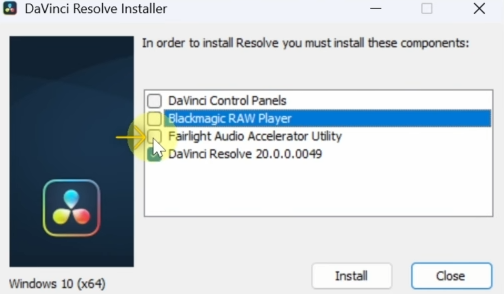
\includegraphics[width=1\textwidth]{assets/davinci-herramientas.png}
        \caption[Tipo Instalacion]{Selección tipo instalación\\ \footnotesize Fuente: Elaboración propia}
        \label{fig:davinci-herramientas}
    \end{figure}

    \item Confirmación de términos y ubicación del programa
    
    Posteriormente al paso indicado antes, se deben acpetar los términos 
    de licencia para usuarios finales (véase Figura~\ref{fig:licencia-davinci}), y se 
    debe seleccionar la ubicación/carpeta del equipo donde se quiere registrar el programa
    (véase Figura~\ref{fig:licencia-davinci}).

    \begin{figure}[H]
        \centering
        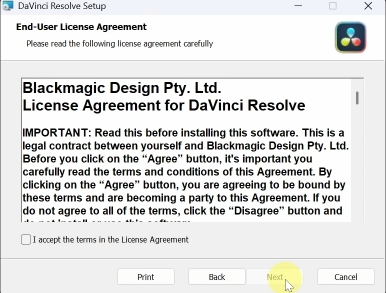
\includegraphics[width=1\textwidth]{assets/licencia-davinci.png}
        \caption[Licencia DaVinci]{Términos de licencia Davinci\\ \footnotesize Fuente: Elaboración propia}
        \label{fig:licencia-davinci}
    \end{figure}

    \begin{figure}[H]
        \centering
        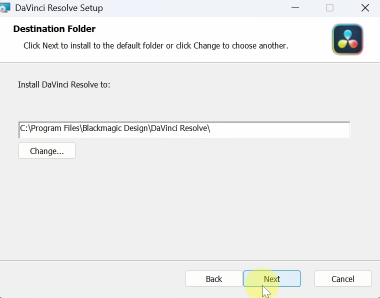
\includegraphics[width=1\textwidth]{assets/ubicacion-davinci.png}
        \caption[Ubicación DaVinci]{Ubicación de registro sobre DaVinci\\ \footnotesize Fuente: Elaboración propia}
        \label{fig:licencia-davinci}
    \end{figure}
\end{itemize}

\subsubsection*{Primera ejecución y configuración básica}
Tras haber configurado la instalación, se puede acceder a la herramienta para comprobar que 
el software en conjunto funciona correctamente, en la Figura~\ref{fig:launcher-davinci} se puede observar 
el arranque inicial de la herramienta cuando se abre.

\begin{figure}[H]
    \centering
    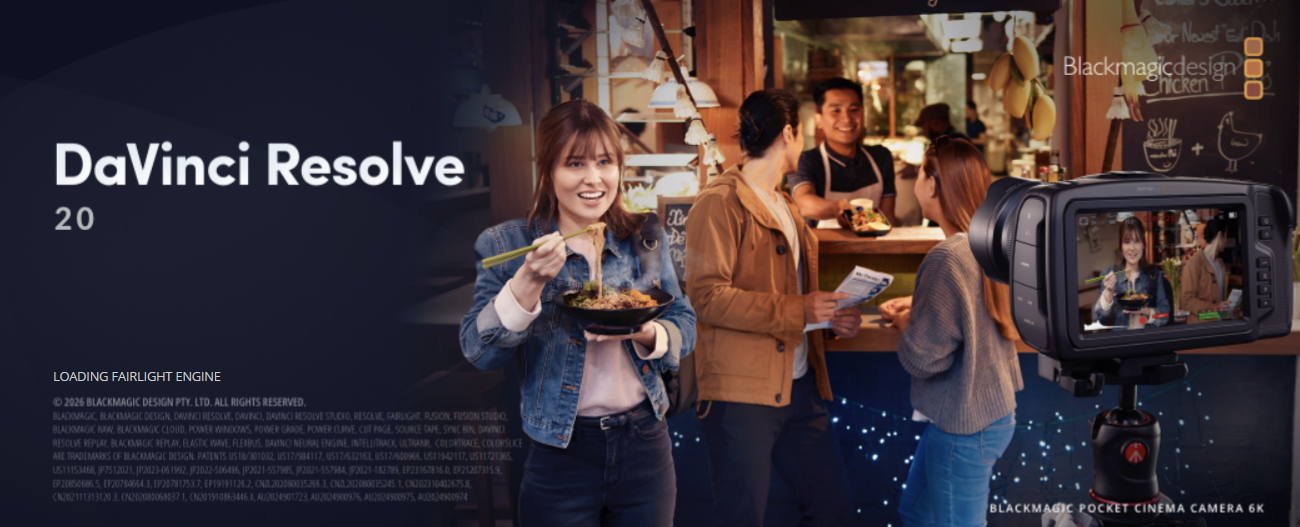
\includegraphics[width=1\textwidth]{assets/launcher-davinci.png}
    \caption[Launcher DaVinci]{Launcher DaVinci Resolve\\ \footnotesize Fuente: Elaboración propia}
    \label{fig:launcher-davinci}
\end{figure}

Si el arranque ha terminado exitosamente, el software procede a mostrar al usuario una pantalla 
de inicio (véase Figura~\ref{fig:inicio-davinci}) caracterizada por las funcionalidades que 
ofrece:

\begin{itemize}
    \item \textbf{Forma de trabajar}
    
    En la parte superior de la pantalla de inicio, se pueden observar \textbf{tres formas} 
    de trabajar sobre un proyecto.

    La primera forma, \textbf{con la que se recomienda trabajar}, mantiene los proyectos en 
    el disco local del equipo. Impidiendo trabajar de forma colaborativa en remoto.

    La segunda forma suele utilizarse más para proyectos empresariales que se suelen configurar 
    dentro de subredes divididas para que un grupo determinado de personas en la empresa, trabajen 
    en esos proyectos de manera colaborativa. Suelen requerir librerías externas de pago y 
    licencias de uso.
    
    La tercera forma sirve para compartir proyectos y entornos de trabajo en la nube, pudiendo 
    acceder cualquier persona que el usuario propietario del proyecto permita, para colaborar 
    de forma remota y parelela en el proyecto. Es necesario contar con librerías externas 
    de pago y licencias de uso.

    \item \textbf{Acciones iniciales}
    
    En la zona central de la pantalla, se suele disponer de los diferentes proyectos que 
    el usuario dispone, en este caso, en su equipo local. Justo en la zona inferior de esta 
    zona, se pueden realizar acciones sobre la \textbf{importación} e 
    \textbf{exportación de proyectos}. Además, la posibilidad de crear un \textbf{nuevo proyecto} o 
    \textbf{abrir} uno existente. 

    Existe una sección de herramientas en la zona centra descrita, pudiendo aplicar filtros 
    y distribución de la visualización de los proyectos disponibles en el caso donde se 
    dispongan de numerosos proyectos, ayudando al usuario a trabjar de una forma más cómoda 
    y poco tediosa.

    \item \textbf{Configuración proyecto}
    
    Al crear un proyecto, para conseguir una mayor calidad de trabajo y resultado final, es 
    necesario tener en consideración las siguientes pautas para la configuración del proyecto 
    creado:

    \begin{enumerate}[label=\arabic*.]
        \item Propiedades del vídeo
        
        Antes de ponerse con la edición de vídeos, es necesario ajustar el entorno del proyecto 
        creado a las propiedades específicas sobre el vídeo con el que se va a trabajar.

        Para ello, es conveniente revisar la anchura y la altura del vídeo, aplicando \textbf{click derecho}
        sobre él, seleccionando la opción \textbf{Propiedades} y accediendo a la sección \textbf{Detalles} 
        en la parte superior de la pestaña (véase Figura~\ref{fig:resolucion-video}).
        Se recomienda tener en cuenta los valores de los atributos desplegados \textbf{Ancho de fotograma} y 
        \textbf{Alto de fotograma} para ajustar la configuración del proyecto.

        \begin{figure}[H]
            \centering
            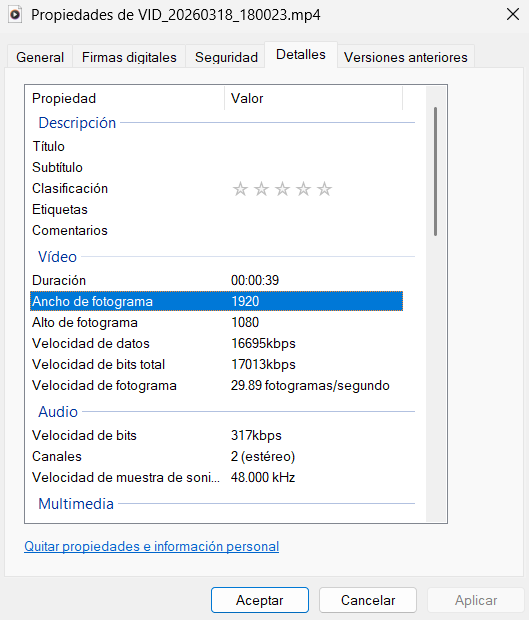
\includegraphics[width=0.6\textwidth]{assets/resolucion-video.png}
            \caption[Resolución Vídeo]{Resolución de vídeo\\ \footnotesize Fuente: Elaboración propia}
            \label{fig:resolucion-video}
        \end{figure}

        \item Configuración interna
        
        Tras obtener el ancho y alto de los fotogramas del vídeo sobre el que se trabajará, 
        es necesario incluirlo en la configuración interna del proyecto para que se adapte al 
        archivo multimedia. 

        En la parte inferior derecha una vez abierto el proyecto creado, se debe acceder al 
        apartado de \textbf{configuración} (véase Figura~\ref{fig:config-proyect}). 
        
        En él, es conveniente modificar, si es necesario la primera sección, llamada 
        \textit{Timeline Format}. Indica la resolución óptima sobre la que se cargará el 
        archivo multimedia con el que trabajar. Por defecto su valor es 1920 x 1080 HD, pero 
        si en el paso anterior se han conseguido valores diferentes a los indicados por 
        defecto, se debe ajustar la resolución manualmente justo debajo de la opción comentada.
        
        Es conveniente maximizar el valor de la propiedad \textit{Timeline frame rate} a 60. Asimismo, 
        con ese mismo valor, la propiedad \textit{Playback frame rate}, pudiendo cargar en una línea 
        de tiempo hasta un total de 60 frames por segundo sobre el vídeo a editar. Versiones de 
        DaVinci de pago pueden permitir más frames por segundo.

        Para el resto de configuración no es necesaria su modificación, pero si es conveniente, se puede 
        adaptar a las necesidades del usuario.

        \begin{figure}[H]
            \centering
            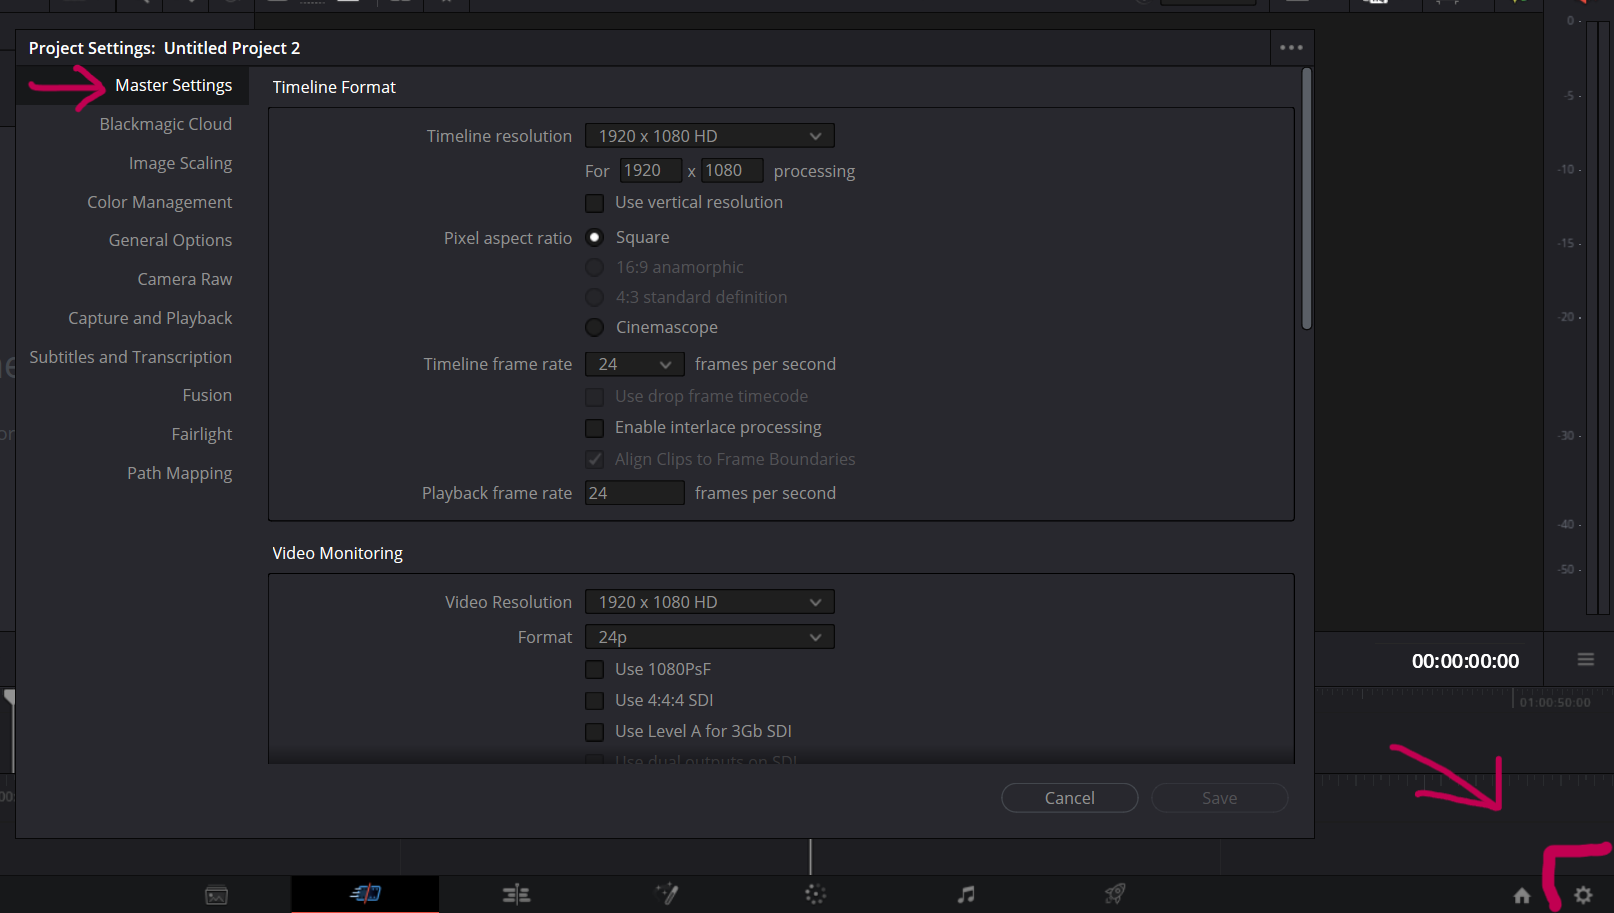
\includegraphics[width=1\textwidth]{assets/config-proyect.png}
            \caption[Configuración Proyecto]{Configuracion proyecto DaVinci\\ \footnotesize Fuente: Elaboración propia}
            \label{fig:config-proyect}
        \end{figure}


    \end{enumerate}
\end{itemize}

\begin{figure}[H]
    \centering
    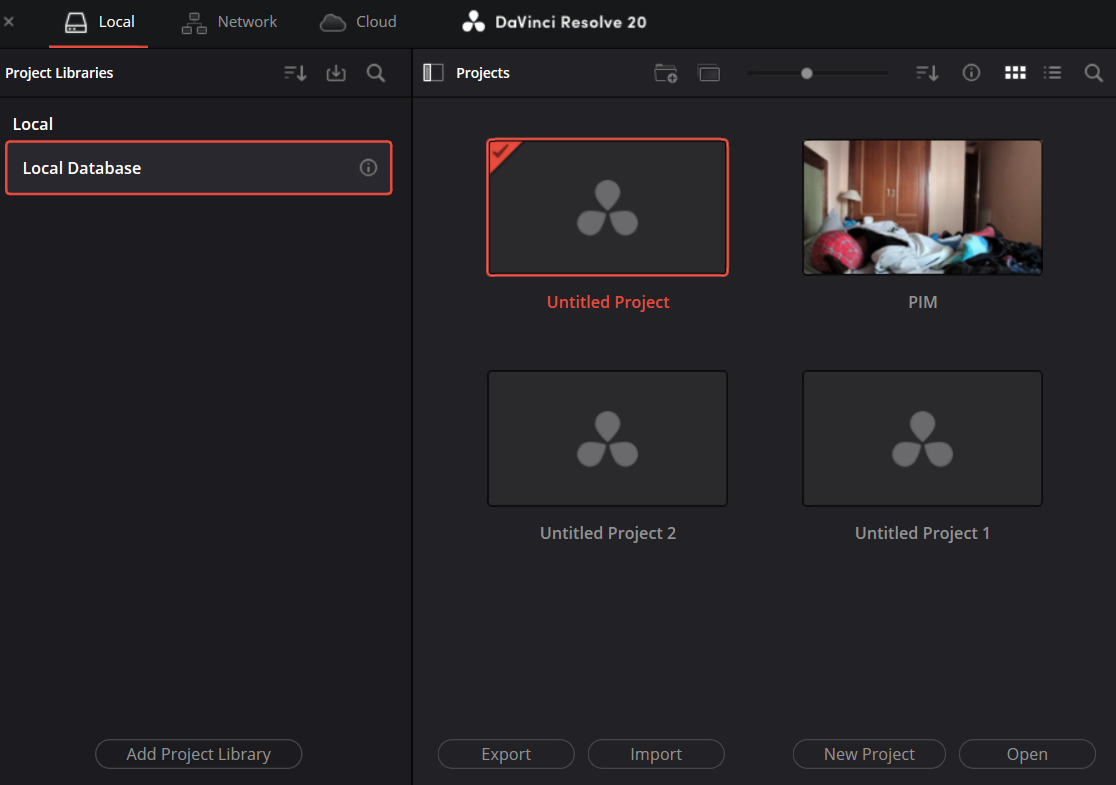
\includegraphics[width=1\textwidth]{assets/pantalla-inicio-dav.png}
    \caption[Pantalla Inicio]{Pantalla Inicio DaVinci\\ \footnotesize Fuente: Elaboración propia}
    \label{fig:inicio-davinci}
\end{figure}

\subsubsection*{Problemas comunes}
